\documentclass[10pt]{article}

% --- Packages ---
\usepackage[utf8]{inputenc}
\usepackage[T1]{fontenc}
\usepackage{lmodern}
\usepackage[margin=1.5cm, top=1.2cm, bottom=1.2cm]{geometry}
\usepackage{amsmath}
\usepackage{graphicx}
\usepackage{booktabs}
\usepackage[table]{xcolor}
\usepackage{float}
\usepackage[font=small, labelfont=bf, skip=2pt]{caption}
\usepackage{enumitem}
\usepackage{titlesec}
\usepackage[colorlinks=true, linkcolor=black, urlcolor=blue]{hyperref}

\graphicspath{{figures/}}
\definecolor{cvred}{HTML}{B2182B}          % shading of the CV table (tables/cv_table.tex)
\definecolor{headpurple}{HTML}{070707}

\setlist[itemize]{leftmargin=1.2em, itemsep=0pt, topsep=1pt, parsep=0pt}
\titleformat{\section}{\large\bfseries\color{headpurple}}{\thesection}{0.6em}{}
\titlespacing*{\section}{0pt}{5pt}{1pt}
\setlength{\parskip}{2pt}
\setlength{\parindent}{0pt}
\setlength{\intextsep}{3pt}
\renewcommand{\arraystretch}{1.08}

\begin{document}

\begin{center}
  {\Large\bfseries (UIC \& NU) Recycled polymer--PAL composites summary}\\[2pt]
  % {\large Project summary and first DoE data}\\[3pt]
  {\small Christian Fernandez \quad$\cdot$\quad \today}
\end{center}
\vspace{-6pt}

%======================================================================
\section{Objective}
%======================================================================
We want a data-driven model that links formulation and processing to the performance of extruded polymer--PAL composites, built on the mechanical data together with the rheology data, while also considering the recycle number. Every reprocessing loop degrades the material, so strength, stiffness, toughness and the flow curve are all expected to drift with the number of recycles. The degradation will be utilized during multi-objective optimization of the mechanical and rheological properties, and predicting how many times a formulation can be recycled before its performance is no longer usable. For the modeling part we are considering  latent-variable Gaussian process for the categorical polymer input that also consider the heteroscedastic noise.

%======================================================================
\section{Inputs, outputs and design of experiments}
%======================================================================
\begin{minipage}[c]{0.64\textwidth}
  \small
  \begin{tabular}{@{}lll@{}}
    \toprule
    \textbf{Input} & \textbf{Type} & \textbf{Values / range} \\
    \midrule
    Polymer system        & categorical & PP+PAL $\cdot$ HDPE+PAL $\cdot$ TPU+PAL \\
    PAL content           & continuous  & 10--50\,\% \\
    Extrusion temperature & continuous  & 180--240\,\textdegree C \\
    Recycle number        & categorical      & 1 / 5 / 10$\times$, on every formulation \\
    \bottomrule
  \end{tabular}

  \vspace{7pt}
  \begin{tabular}{@{}lll@{}}
    \toprule
    \textbf{Output} & \textbf{Units} & \textbf{Test} \\
    \midrule
    UTS                         & MPa                     & tensile, $\geq 3$ replicates \\
    Young's modulus (stiffness) & MPa                     & tensile \\
    Toughness                   & MJ/m\textsuperscript{3} & tensile \\
    Strain at break             & --                      & tensile \\
    Viscosity / flow curve      & Pa$\cdot$s              & rheometer, window 0.1--10\,s$^{-1}$ \\
    \bottomrule
  \end{tabular}
\end{minipage}\hfill
\begin{minipage}[c]{0.30\textwidth}
  \centering
  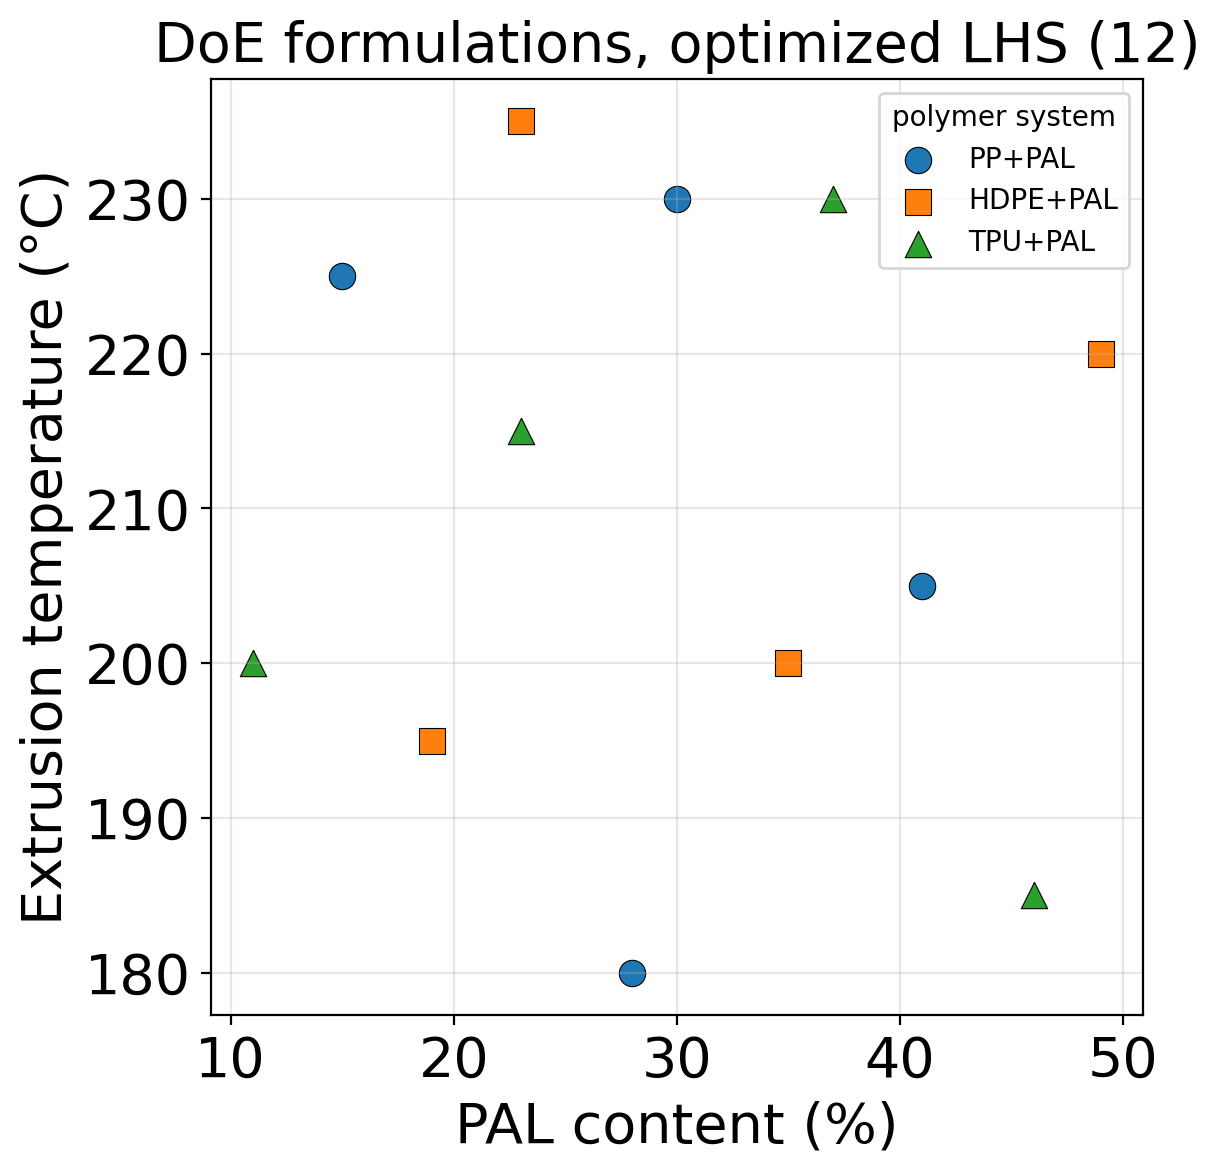
\includegraphics[width=\linewidth]{doe_formulations.png}
  \captionof{figure}{The 12 DoE formulations.}\label{fig:doe}
\end{minipage}

\vspace{4pt}
The formulation factors are sampled with an optimized Latin hypercube: \textbf{12 formulations}, four per polymer (Fig.~\ref{fig:doe}). Every formulation is carried through the whole 1 / 5 / 10$\times$ recycle, giving \textbf{36 measurements} plus repeated samples.

%======================================================================
\section{First DoE data}
%======================================================================
The initial dataset contains only tensile measurements from 30 specimens, representing 9 of the 12 planned formulations. Both the PP+PAL and HDPE+PAL systems are fully sampled with 3 to 5 replicates each, whereas the TPU+PAL system currently includes only a single specimen; rheological data has not yet been collected. As shown in Figures \ref{fig:factors} and \ref{fig:space}, UTS ranges mainly from 6 to 14 MPa and Young's modulus from 350 to 810 MPa. Increasing the PAL content decreases both properties in PP and HDPE alike, with optimal performance observed at low PAL concentrations extruded at approximately 195–200\textdegree C. Notably, the single TPU specimen exhibits elastomer behavior, yielding a toughness of 2.2 MJ/m\textsuperscript{3}, which is roughly five times greater than any other formulation. Within a given polymer class, UTS and toughness are not competing objectives as it can be observed on Figure \ref{fig:corr}. The trade-offs exist between Young's modulus and toughness, and in the selection of the base polymer (such as TPU).

\begin{figure}[H]
  \centering
  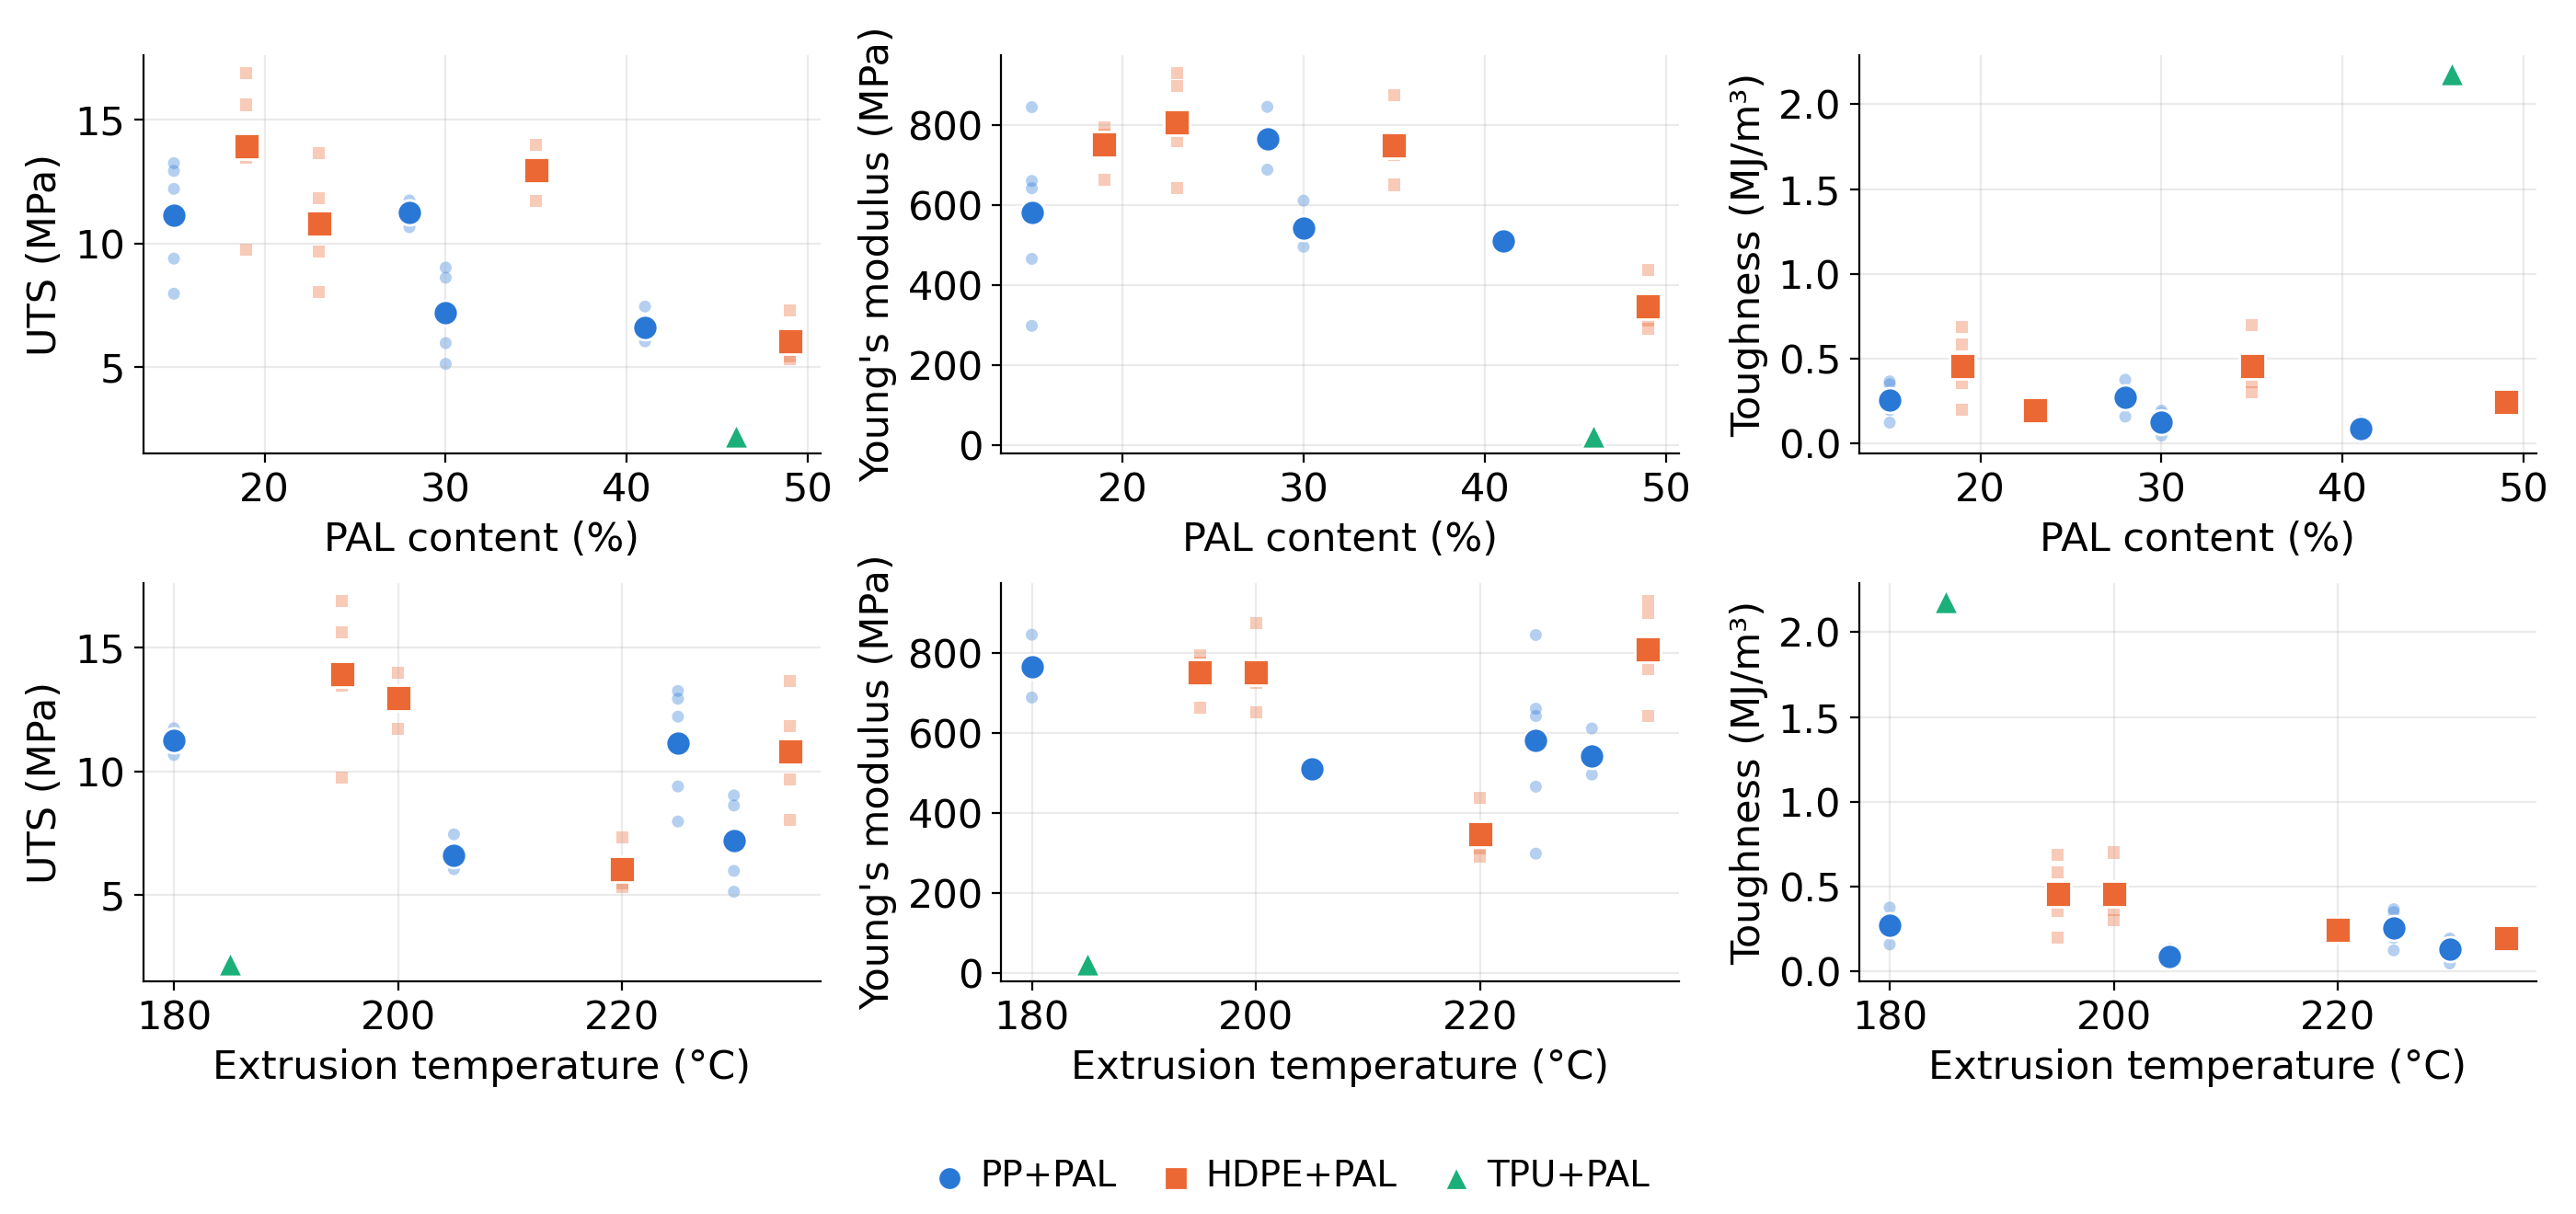
\includegraphics[width=0.80\textwidth]{doe_tensile_props_vs_factors.png}
  \caption{Tensile properties against the two continuous factors.}
  \label{fig:factors}
\end{figure}



\begin{figure}[H]
  \centering
  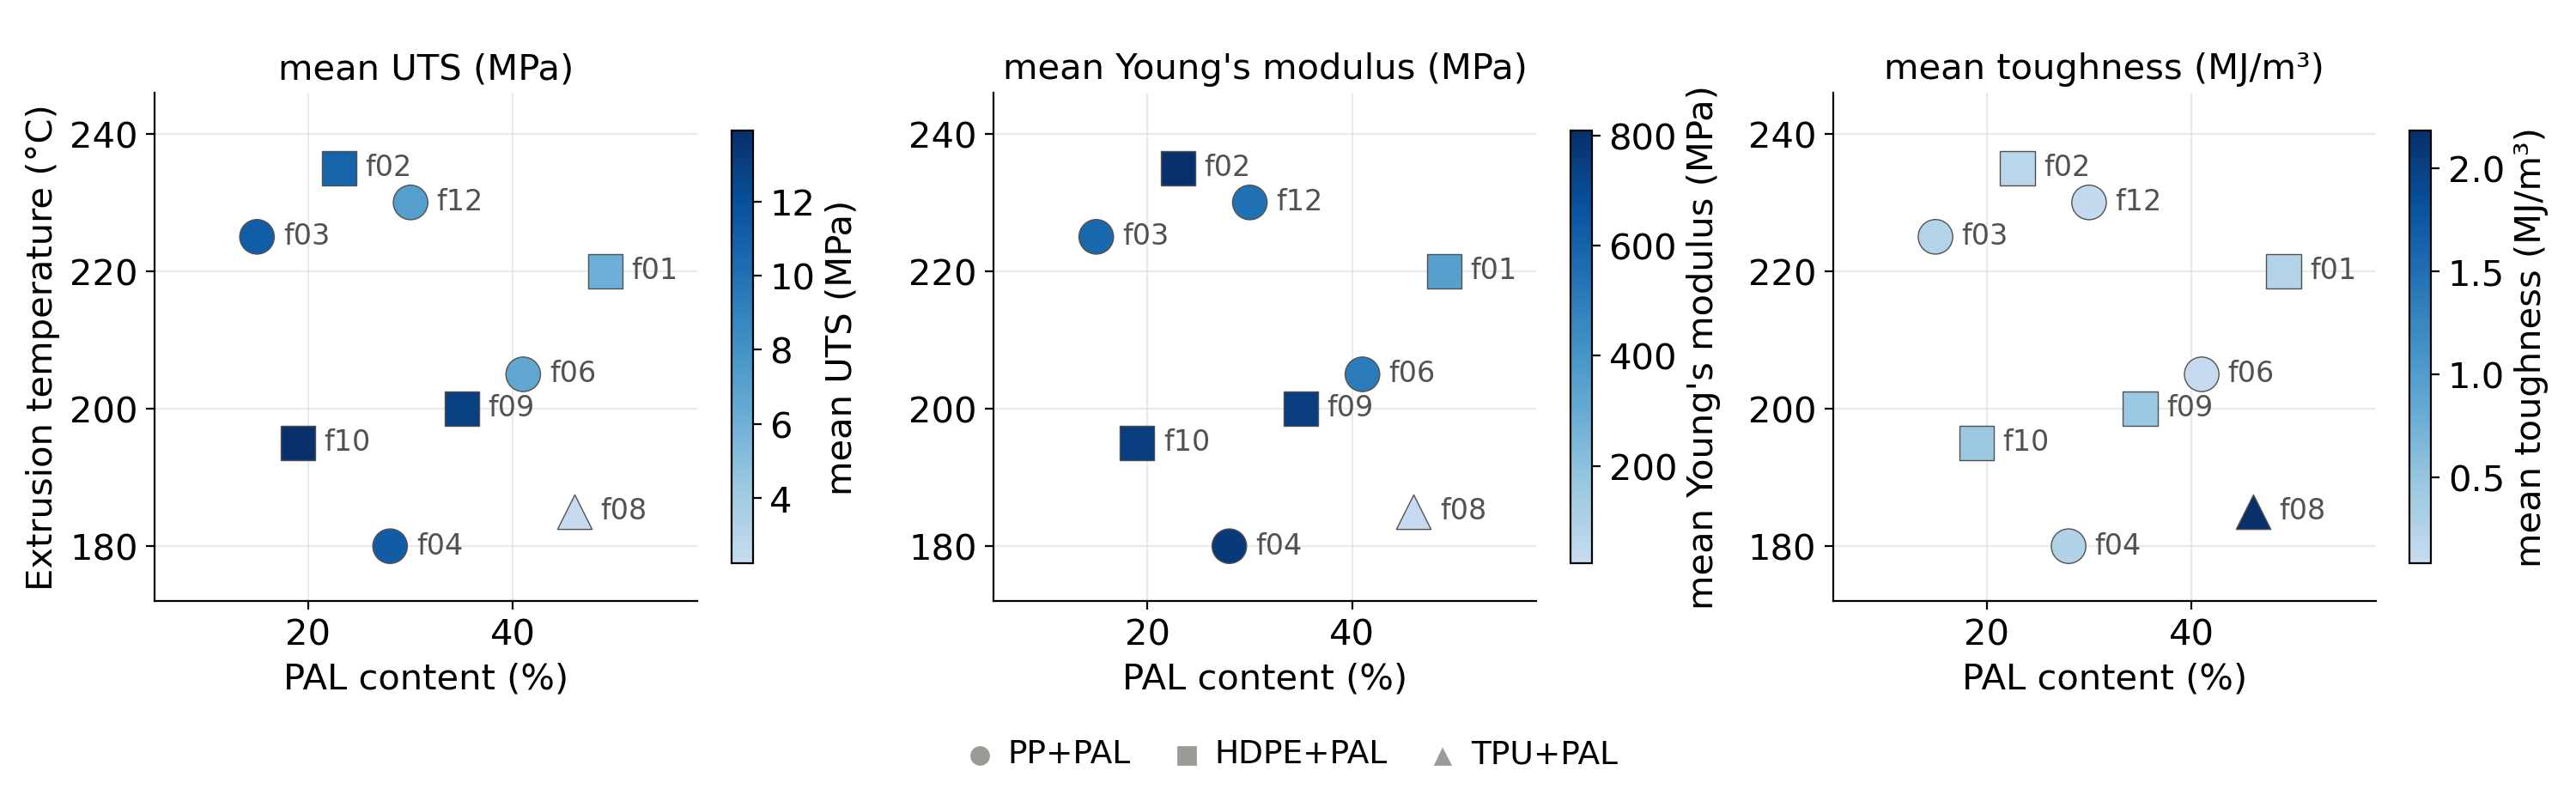
\includegraphics[width=0.85\textwidth]{doe_tensile_design_space.png}
  \caption{Formulation means placed in the design space.}
  \label{fig:space}
\end{figure}

\begin{figure}[H]
  \centering
  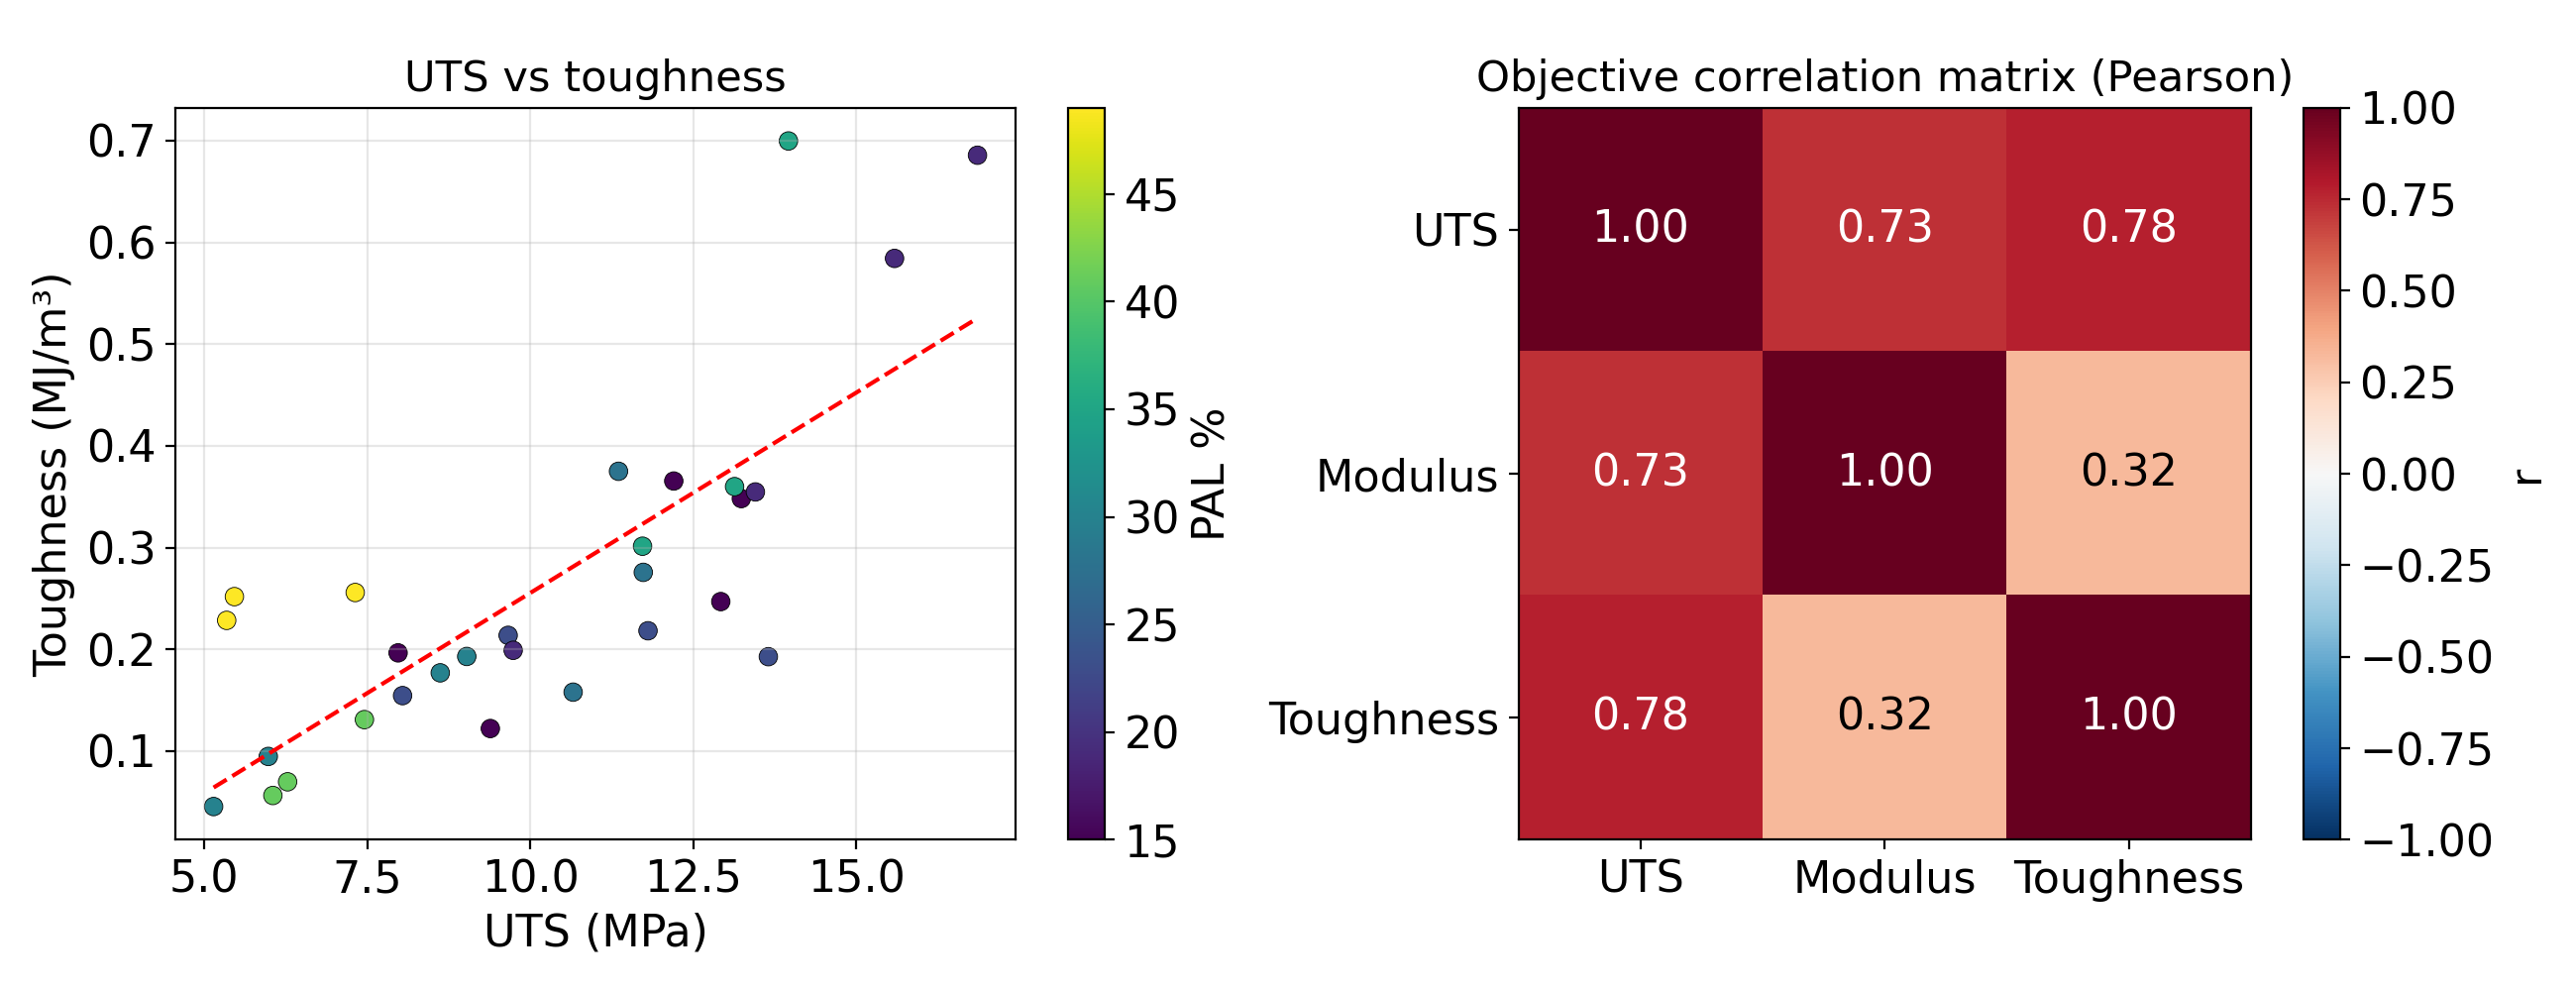
\includegraphics[width=0.70\textwidth]{doe_tensile_uts_toughness_correlation.png}
  \caption{UTS vs.\ toughness per specimen, and the objective correlation matrix (PP+PAL and HDPE+PAL, $n = 29$).}
  \label{fig:corr}
\end{figure}

%======================================================================
\section{Replicate noise}
%======================================================================
\begin{table}[H]
  \centering\footnotesize\renewcommand{\arraystretch}{1.0}
  % generated by build_assets.py from processed_data/tensile_doe/tensile_doe_summary.csv
\begin{tabular}{llrrr rr rr rr}
\toprule
 & & PAL & $T_\mathrm{extr}$ & & \multicolumn{2}{c}{Young's modulus} & \multicolumn{2}{c}{UTS} & \multicolumn{2}{c}{Toughness} \\
\cmidrule(lr){6-7}\cmidrule(lr){8-9}\cmidrule(lr){10-11}
Form. & Polymer & (\%) & (\textdegree C) & $n$ & mean (MPa) & CV (\%) & mean (MPa) & CV (\%) & mean (MJ/m\textsuperscript{3}) & CV (\%) \\
\midrule
f01 & HDPE+PAL & 49 & 220 & 3 & 347 & \cellcolor{cvred!34}22.9 & 6.0 & \cellcolor{cvred!27}18.3 & 0.25 & \cellcolor{cvred!9}6.0 \\
f02 & HDPE+PAL & 23 & 235 & 4 & 809 & \cellcolor{cvred!24}16.4 & 10.8 & \cellcolor{cvred!33}22.7 & 0.19 & \cellcolor{cvred!22}14.9 \\
f03 & PP+PAL & 15 & 225 & 5 & 583 & \cellcolor{cvred!52}35.7 & 11.1 & \cellcolor{cvred!31}21.0 & 0.26 & \cellcolor{cvred!59}\color{white}40.0 \\
f04 & PP+PAL & 28 & 180 & 3 & 767 & \cellcolor{cvred!15}10.2 & 11.2 & \cellcolor{cvred!7}4.9 & 0.27 & \cellcolor{cvred!59}\color{white}40.3 \\
f06 & PP+PAL & 41 & 205 & 3 & 510 & \cellcolor{cvred!5}3.6 & 6.6 & \cellcolor{cvred!17}11.4 & 0.09 & \cellcolor{cvred!68}\color{white}46.3 \\
f08 & TPU+PAL & 46 & 185 & 1 & 24 & -- & 2.2 & -- & 2.18 & -- \\
f09 & HDPE+PAL & 35 & 200 & 3 & 751 & \cellcolor{cvred!22}15.2 & 12.9 & \cellcolor{cvred!13}8.8 & 0.45 & \cellcolor{cvred!70}\color{white}47.4 \\
f10 & HDPE+PAL & 19 & 195 & 4 & 751 & \cellcolor{cvred!12}8.0 & 13.9 & \cellcolor{cvred!33}22.4 & 0.46 & \cellcolor{cvred!71}\color{white}48.3 \\
f12 & PP+PAL & 30 & 230 & 4 & 544 & \cellcolor{cvred!13}8.9 & 7.2 & \cellcolor{cvred!39}26.7 & 0.13 & \cellcolor{cvred!80}\color{white}54.5 \\
\bottomrule
\end{tabular}

  \caption{Coefficient of variation (std/mean) across replicates, one shading scale for all CV columns; f08 has one specimen.}
  \label{tab:cv}
\end{table}

The experimental noise is significant and heteroscedastic, with coefficients of variation reaching 36\,\% for modulus, 27\,\% for UTS, and 55\,\% for toughness (Table~\ref{tab:cv}). This variance changes across inputs and is likely affected by filament diameter variations (1.40--2.05\,mm) and heterogeneous mixing among polymers.

\end{document}
